\section{Modeling Metabolites using EKF}
\label{Modeling Metabolites using EKF}
\label{chap:EKF_Meskin}

\noindent This example is inspired by research that models the biological pathway of metabolites, which are molecules that are the byproduct of the body's metabolism. This model contains four different states, or metabolites, which contain 18 unknown parameters \cite{article5}. Unlike the original research, which had datasources of their own, this example will simulate data by using a built-in ODE solver on Matlab. The dataset used to generate these results are included along with the code in the appendix. Ultimately, the goals of this example is to demonstrate how the EKF can be applied, how the EKF can correct for multiple variables or states, and how the EKF can be used for parameter fitting. \\ 

\noindent In this example, the four metabolites, or states, have the following differential equations:
\begin{align*}
\dot x_1 &= \alpha_1 x_3^{g_{13}}  - \beta_1 x_1^{h_{11}}, \\
\dot x_2 &= \alpha_2 x_1^{g_{21}} - \beta_2 x_2^{h_{22}}, \\
\dot x_3 &= \alpha_3 x_2^{g_{32}} - \beta_3 x_3^{h_{33}} x_4^{h_{34}}, \\
\dot x_4 &= \alpha_4  x_1^{g_{41}} - \beta_4 x_4^{h_{44}},
\end{align*}
where there are 18 unknown parameters ($\alpha_1, \hdots, \alpha_4, \beta_1, \hdots, \beta_4, g_{13}, g_{15}, g_{21}, \\ g_{32}, g_{41}, h_{11}, h_{22}, h_{33}, h_{34}, h_{44} $) and the state vector is given by $x= [x_{1}, x_{2}, x_{3}, x_{4}]^T$. For now, we will use the true value of these parameters (which can be found in \cite{article5}), but later on the EKF will be applied for parameter estimation. In both the original example as well as this one, sampling time will be 0.1 seconds for 5 seconds, totaling 50 UKF estimates. \\



\clearpage
\subsubsection{Implementing EKF}

Recall that implementing the EKF requires initializing the model, generating a prediction, and correcting the prediction. Below outlines the process of how the EKF can be applied for a single time step. Applying the EKF to multiple time steps is simulated on Matlab, and the code for doing so can be found in the appendix.

\begin{enumerate}
\item The model is initialized by setting the state variable to $x_0 = [4, 1, 3, 4]^T$, which is very close to the true values of the system. Since the initialized state has values near the true value, the state covariance can also be set to a lower value of $P_0 = .01I$. 
\item The next step is to generate a prediction. To do so, the system must be discretized into time steps. The system is given in a continuous state space in the form of $\dot x = Ax$, and can be discretized by converting it into the form $\dot x = e^{At}x$. However, in this system, calculating the matrix exponential is computationally intense (taking days to run on a single iteration on Matlab). Therefore, the Euler method will be used with a time step of 0.05 seconds, resulting in
\begin{align*}
 x_{1|0} &=  x_{0|0} + 0.05  * f(x) \\ \\
&= \begin{bmatrix}
4 \\
1\\
3 \\
4
\end{bmatrix} + 0.05
\begin{bmatrix}
 \alpha_1 3^{g_{13}} - \beta_1 4 ^{h_{11}} \\
 \alpha_2 4^{g_{21}} - \beta_2 1^{h_{22}} \\
 \alpha_3 1^{g_{32}} - \beta_3 3^{h_{33}} 4^{h_{34}} \\
\alpha_4  4^{g_{41}} - \beta_4 4^{h_{44}}
\end{bmatrix} \\ \\
&=\begin{bmatrix}
3.4152 \\
1.6500 \\
2.5786 \\
3.2906
\end{bmatrix}.
\end{align*}

\item Finally, the prediction can be corrected. Calculate $F$, the jacobian of the nonlinear transformation $f=[\dot x_1, \dot x_2, \dot x_3, \dot x_4]^T$, and $H$, the Jacobian of the nonlinear observation function $h=[\dot x_1, \dot x_2, \dot x_3, \dot x_4]^T$, as follows
\begin{align*}
F = H = 
\begin{bmatrix}
-\beta_1 h_{11} x_1^{h_{11}-1} & 0 & x_5 x_3 g_{13} ^{g_{13}-1}& 0 \\
\alpha_2  g_{21} x_1^{g_{21}-1} & -\beta_2 h_{22} x_2^{h_{22}-1}&0&0\\
0&\alpha_3 g_{32} x_2^{g_{32}-1} & -\beta_3 h_{33} x_3^{h_{33}-1} x_4^{h_{34}}&-\beta_3 h_{34} x_4^{h_{34}-1} x_3^{h_{33}}\\
\alpha_4 g_{41} x_1^{g_{41}-1}&0&0&-\beta_4 h_{44} x_4^{h_{44}-1}
\end{bmatrix}.
\end{align*}




\noindent  $H$ should be adjusted according to how many states are being corrected. For instance, if correction is being done for all states, $H$ should remain as it is above. However, if only the first state is being corrected, then $h = [\dot x_1]$ and $H = [-\beta_1 h_{11} x_1^{h_{11}-1},  0,  x_3 g_{13} ^{g_{13}-1}, 0 ]$. \\

\noindent Assuming that the first state is the only state being corrected, $F$ and $H$ are used to calculate the Kalman Gain, which is 
\begin{align*}
K_1 = 
\begin{bmatrix}
.05402 & -.0370 & .0465 & .0149
\end{bmatrix}^T.
\end{align*}

\noindent Additionally, the prediction can be transformed in order to compare it with incoming system measurement. In the case where only the first state is being predicted, the prediction is transformed by applying the nonlinear observation function to the prediction. Similar to generating the prediction, this can be done by using Euler's method to discretize the system, resulting in
\begin{align*}
y_{1} &=  x_{1,1|0} + 0.05 * h(x_{1|0}) \\ 
&=3.4152  + 0.05(\alpha_1 2.5786 ^{g_{13}} - \beta_1 3.4152  ^{h_{11}} )=
2.9600.
\end{align*}

\noindent This transformed value is quite close to the measured value of 3.1126, meaning that in the first time step, the residual is approximately .15. Recall that the measured value was simulated on Matlab and can be found in the appendix.\\

\noindent Finally, the prediction can be corrected, resulting in
\begin{align*}
 x_{1|1}&=
  x_{1|0} + K_1 (y_1 - \hat y_1) =
\begin{bmatrix}
3.5751\\
1.5404 \\
2.7162 \\
3.3346
\end{bmatrix}.
\end{align*}

\end{enumerate}


\begin{figure}[ht]
    \centering
    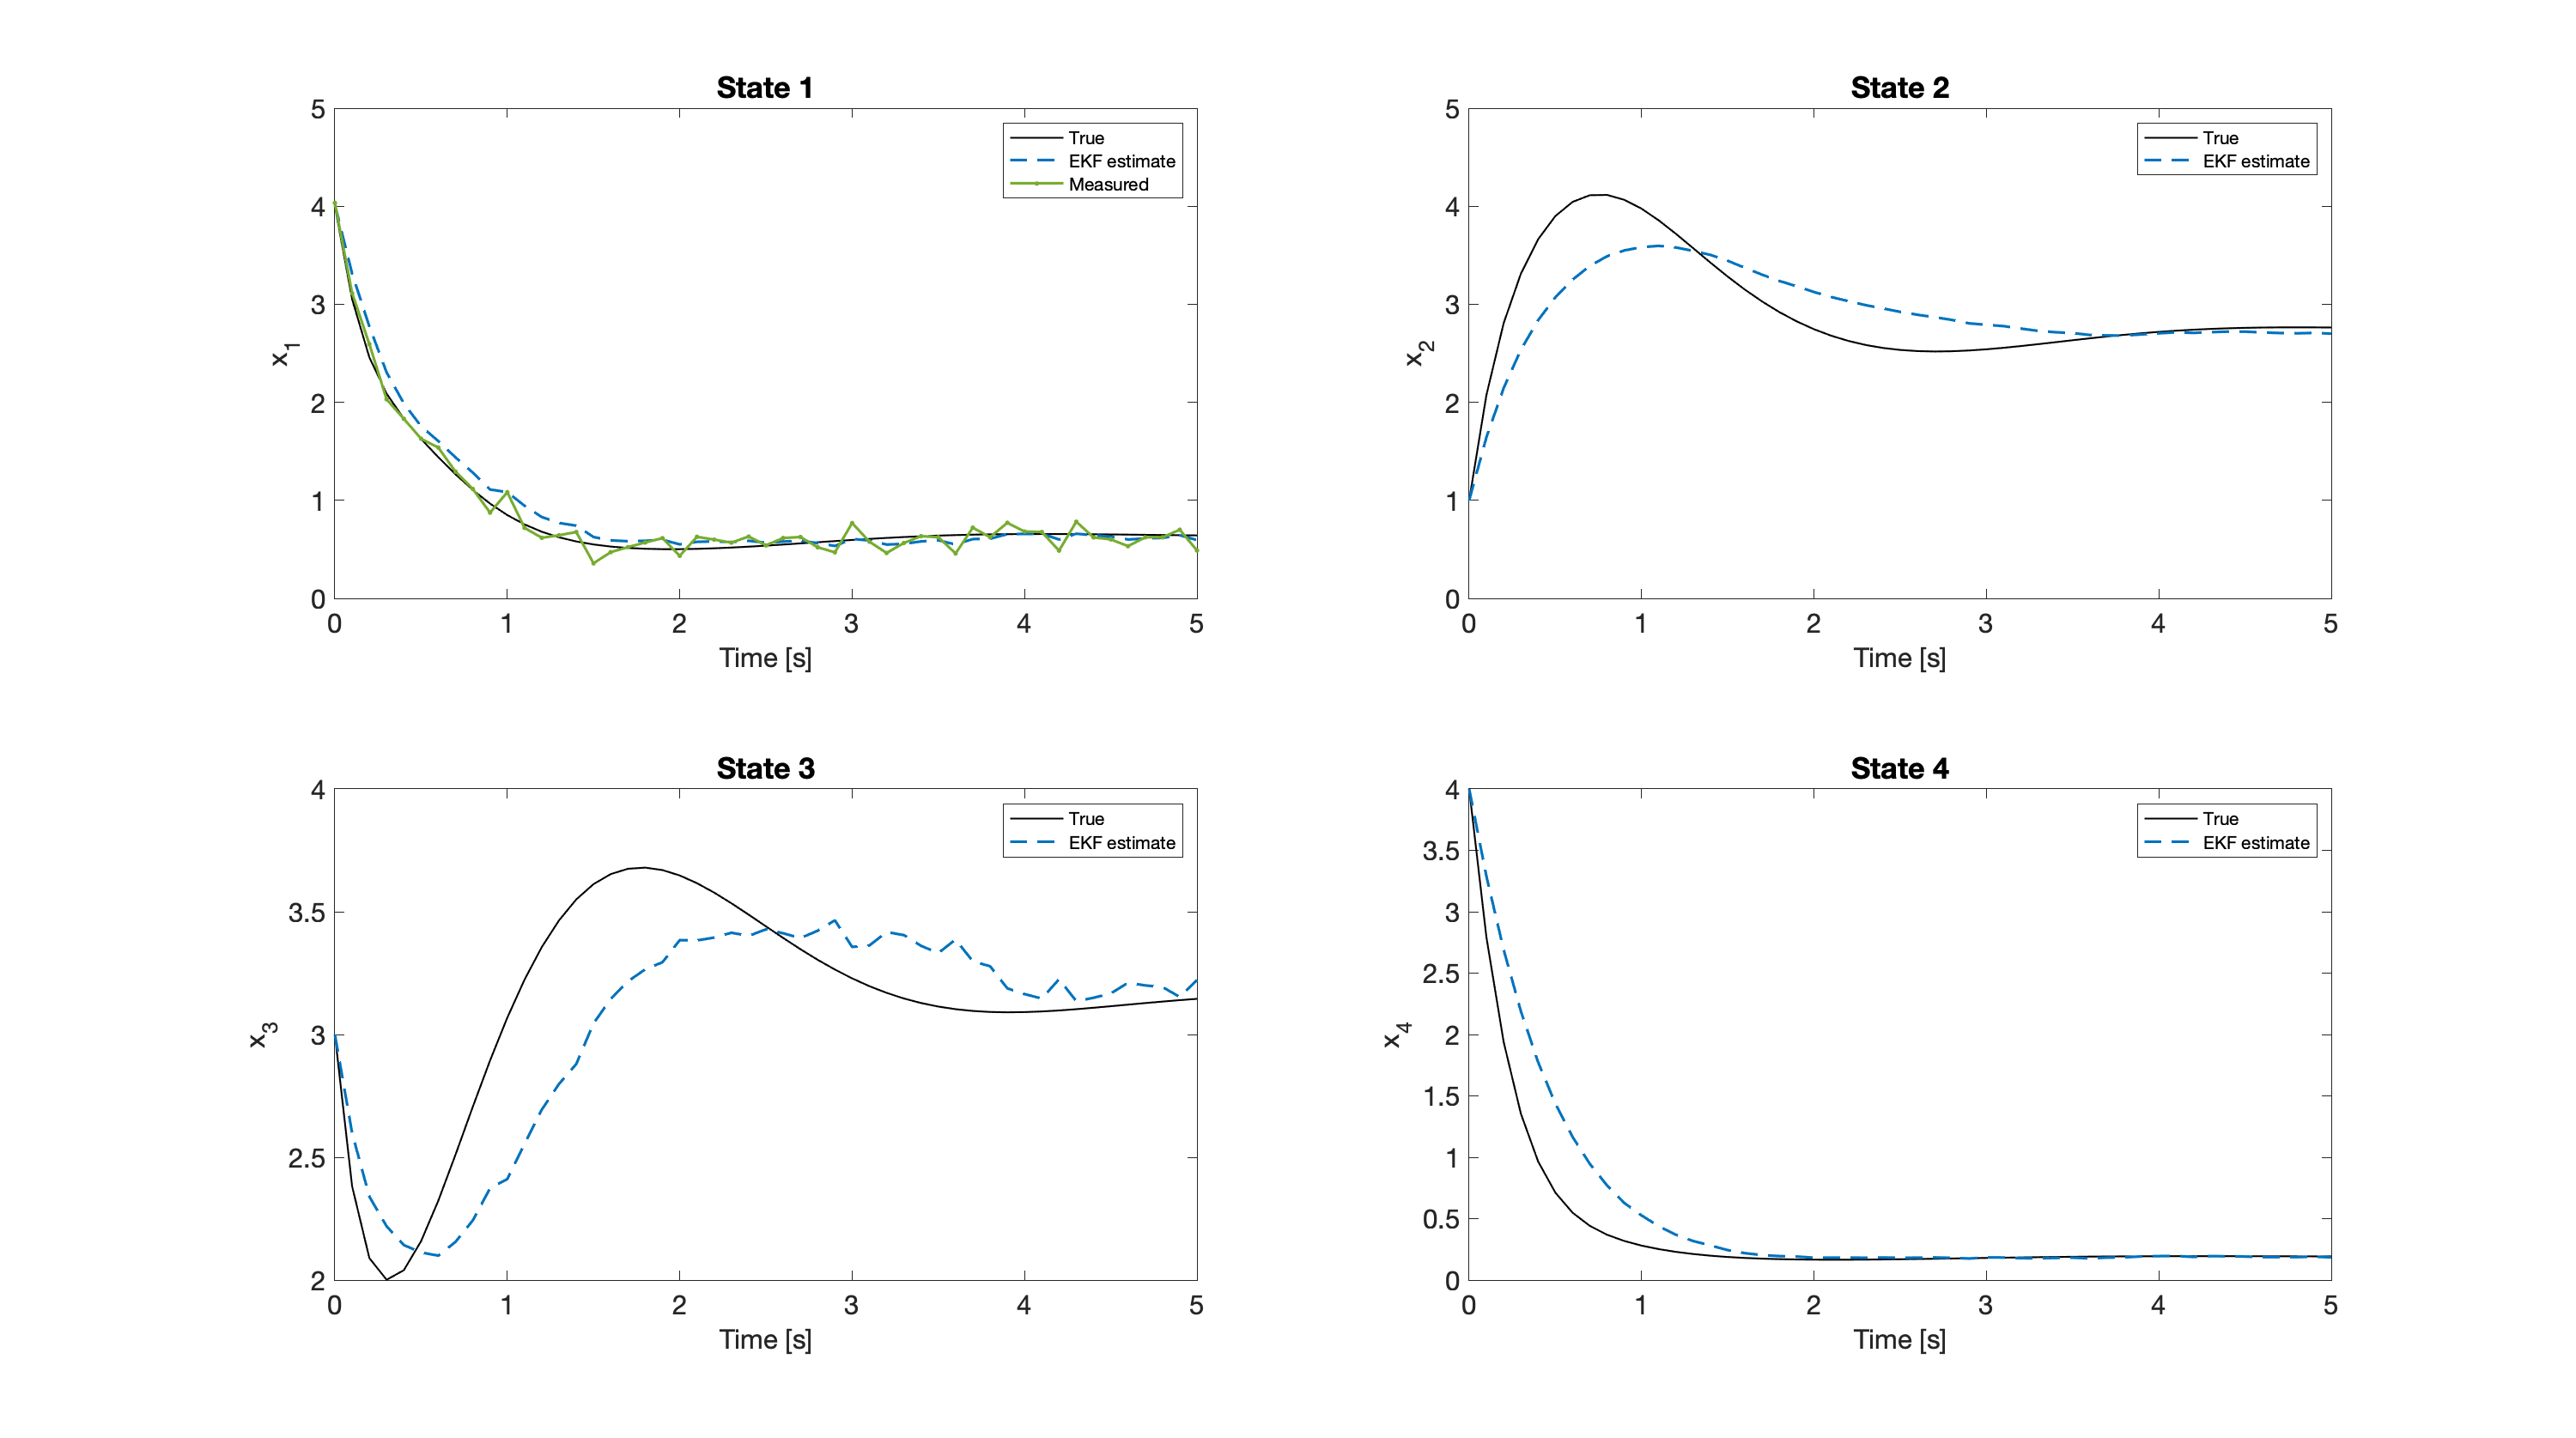
\includegraphics[scale = 0.3]{EKF_1state.png}
    \caption{Implementing EKF with correction applied to State 1 and initialized with states $[4, 1, 3, 4]^T$.}
    \label{fig:EKF_1state}
	\vspace*{\floatsep}%
    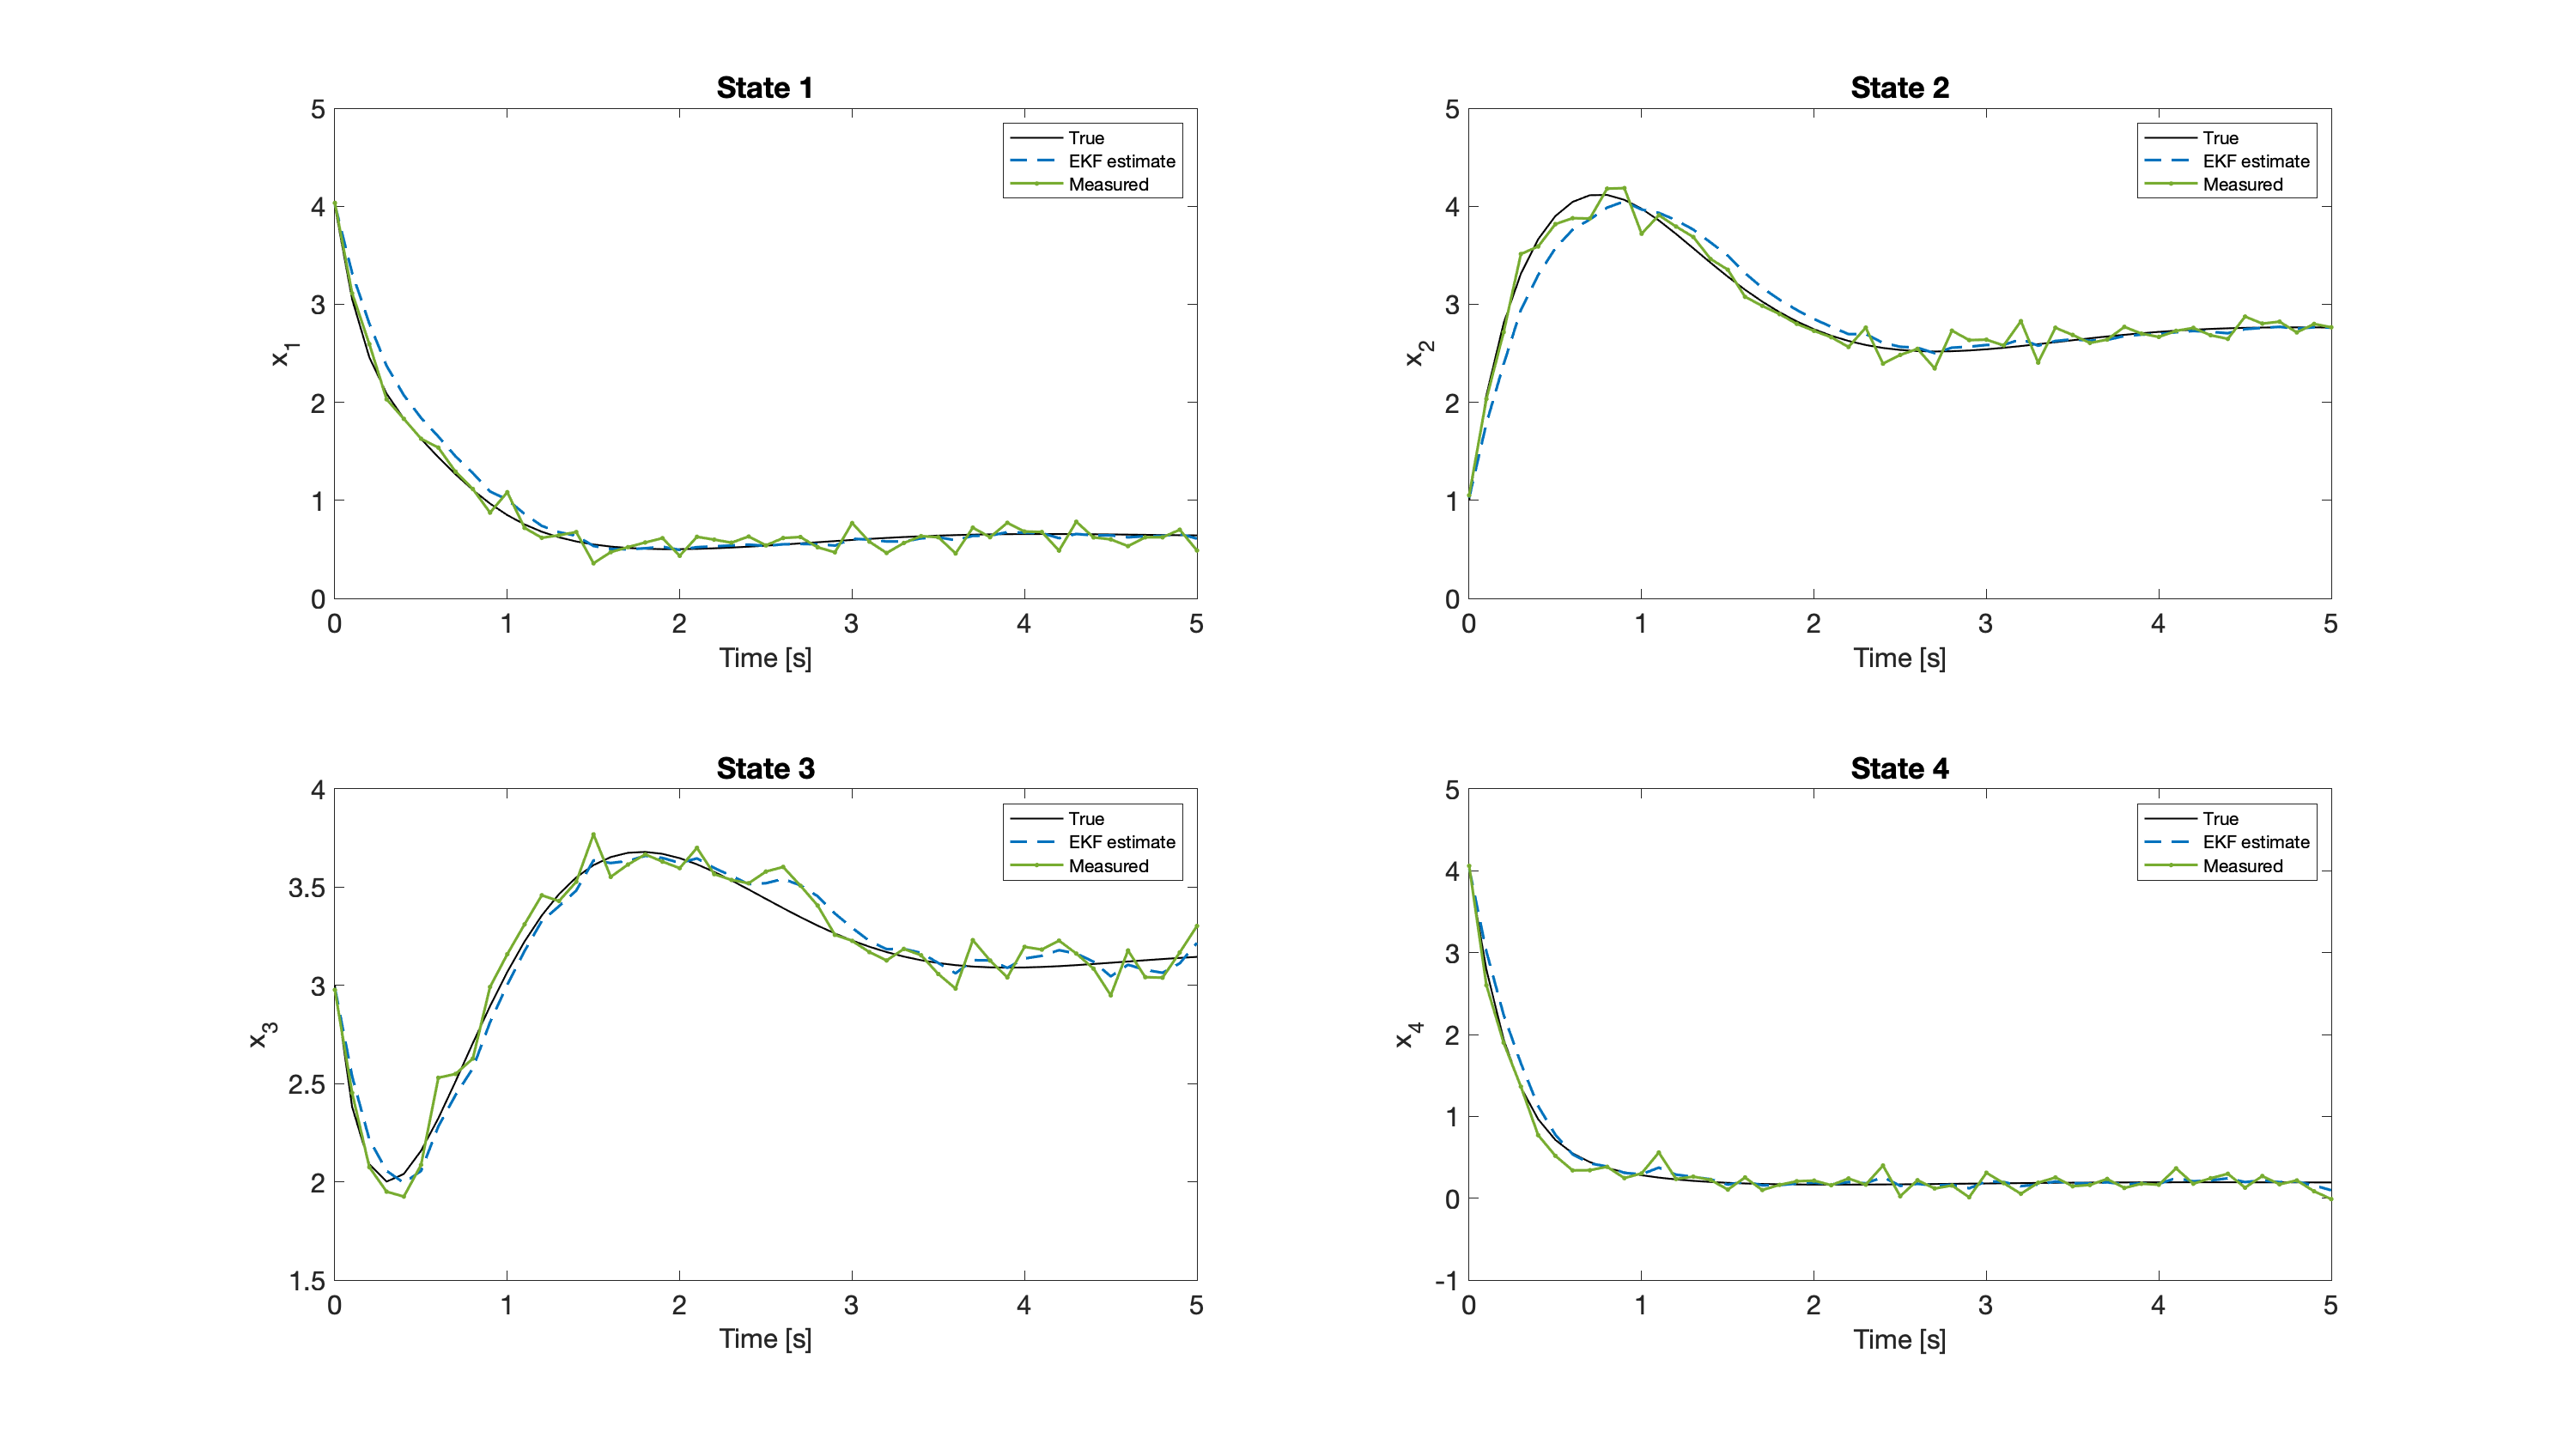
\includegraphics[scale = 0.3]{EKF_4state.png}
    \caption{Using EKF with correction applied to all states using a model initialized with states $[4, 1, 3, 4]^T$.}
    \label{fig:EKF_4state}
\end{figure}



\noindent Applying the EKF for 50 time steps by repeating steps 2 and 3 on Matlab results in figure \ref{fig:EKF_1state}. Multiple state correction is similar to the implementation above. The only difference is in the correction step. Notice the improvement in performance when all states are being corrected, as seen in fig \ref{fig:EKF_4state}.  \\

\noindent For more examples on applying the EKF and MATLAB code, the following can be referenced \cite{cao_2008, article7}.






\clearpage
\subsubsection{EKF Parameter Estimation}
The EKF (as well as other versions of the Kalman Filter), can be utilized for parameter estimation. There are many methods of parameter estimation, which include using dual techniques. In fact, there is a nonlinear version of the Kalman Filter, called the Dual Unscented Kalman Filter, that was designed in order to simultaneously monitor state and parameter values. Though this thesis does not explore these methods, more information can be found in \cite{inbook, article6}. In particular, this thesis explores the use of joint parameter estimation. This technique involves creating new states for each of the unknown parameters. \\ 

\noindent In this example, the goal is to use the EKF to find parameter values that best fit this model to its true states. This example continues to use the metabolites system with the goal of estimating parameter $\alpha_1$. Begin by declaring $\alpha_1$ as a separate state. The new set of differential equations for this 5 state system is given by
\begin{align*}
\dot x_1 &= x_5 x_3^{g_{13}} - \beta_1 x_1^{h_{11}}, \\
\dot x_2 &= \alpha_2 x_1^{g_{21}} - \beta_2 x_2^{h_{22}}, \\
\dot x_3 &= \alpha_3 x_2^{g_{32}} - \beta_3 x_3^{h_{33}} x_4^{h_{34}}, \\
\dot x_4 &= \alpha_4  x_1^{g_{41}} - \beta_4 x_4^{h_{44}}\\
\dot x_5 &= 0.
\end{align*}


\noindent The ODE for $x_5$ is 0, because $x_5$ is a parameter, or constant, and does not change overtime. In this 5 state system, the nonlinear state transition function is equal to $f = [\dot x_1, \dot x_2, \dot x_3, \dot x_4, \dot x_5]^T$. By applying the EKF to this system while correcting for all 5 states, the EKF performs well, as shown in ~\ref{fig:EKF_1param}.

\begin{figure}[h]
    \centering
    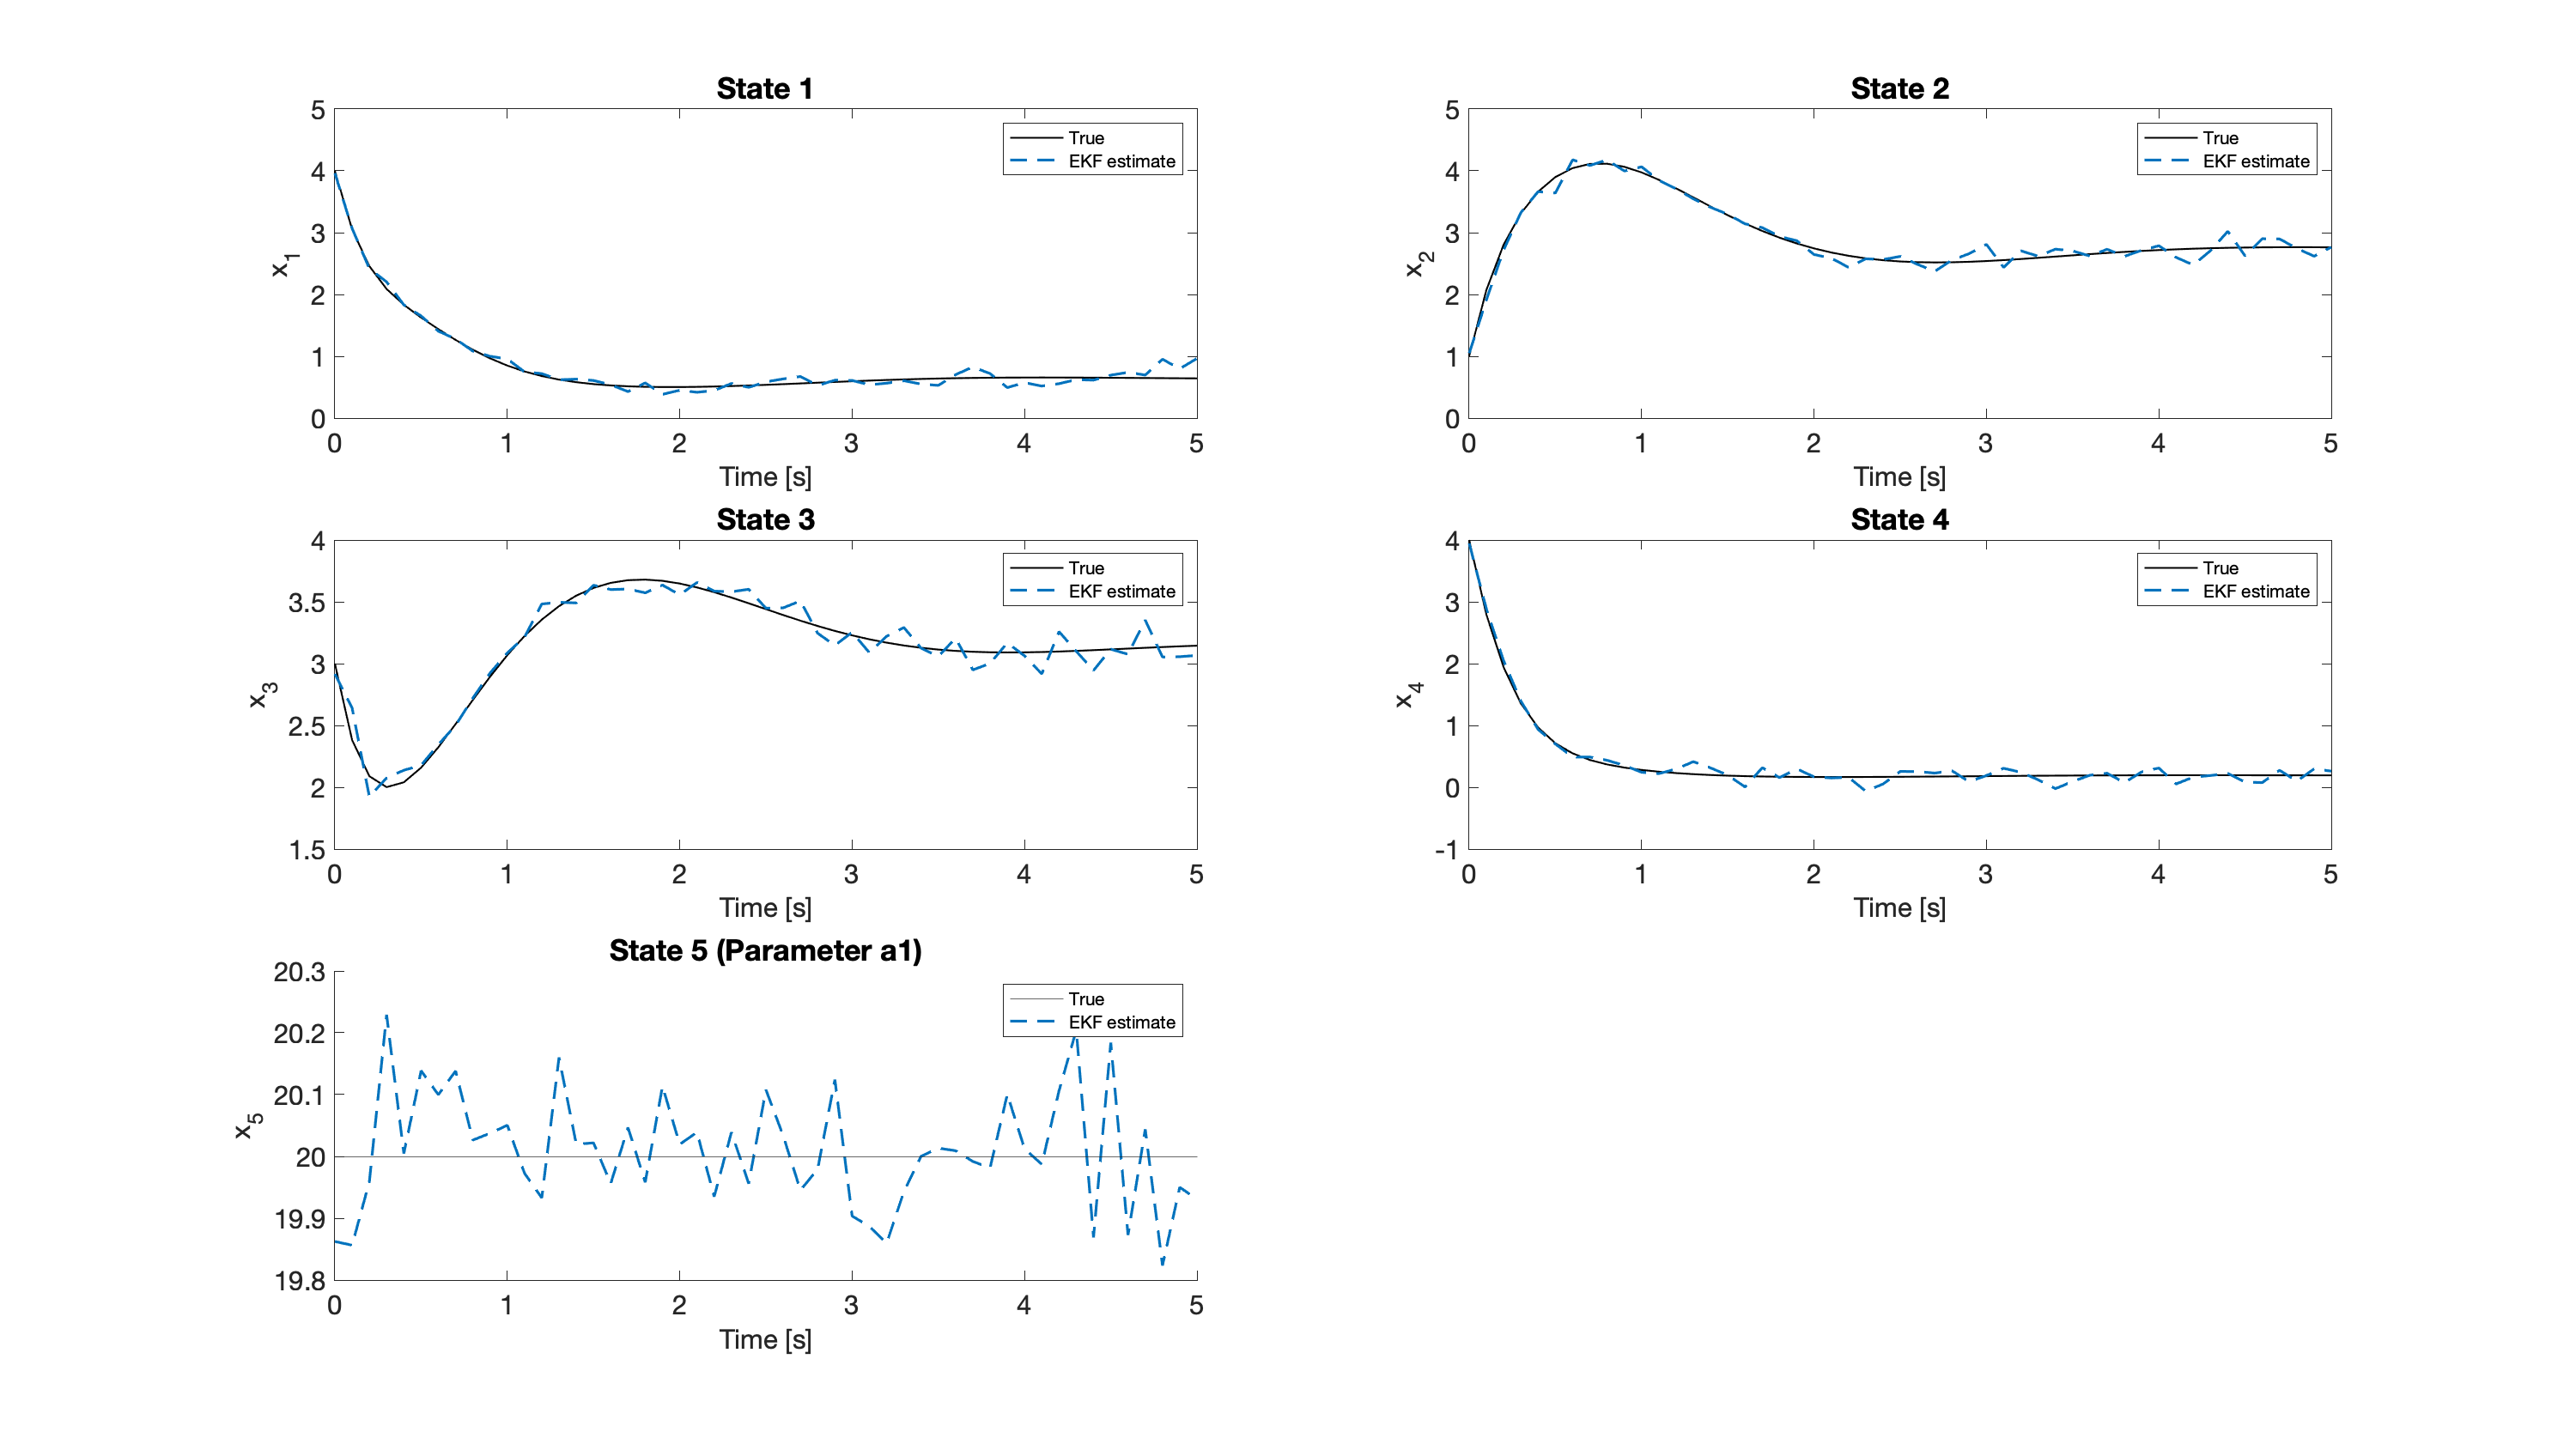
\includegraphics[scale = 0.3]{EKF_1param.png}
    \caption{Results obtained by implementing the EKF with parameter estimation of $\alpha_1$. The model is initialized with $[4, 1, 3, 4, 20]^T$, which is close to the true initial value of the system. While not depicted in this visual, the model still performs well when initialized with values further from the true system values. }
    \label{fig:EKF_1param}
\end{figure}

\comment{
The jacobian of $f$, or $F$ is given by
$$
\scriptsize{
\begin{bmatrix}
-\beta_1 h_{11} x_1^{h_{11}-1} & 0 & x_5 x_3 g_{13} ^{g_{13}-1}& 0 & x_3^{g_{13}}\\
\alpha_2  g_{21} x_1^{g_{21}-1} & -\beta_2 h_{22} x_2^{h_{22}-1}&0&0&0 \\
0&\alpha_3 g_{32} x_2^{g_{32}-1} & -\beta_3 h_{33} x_3^{h_{33}-1} x_4^{h_{34}}&-\beta_3 h_{34} x_4^{h_{34}-1} x_3^{h_{33}}&0\\
\alpha_4 g_{41} x_1^{g_{41}-1}&0&0&-\beta_4 h_{44} x_4^{h_{44}-1}&0\\
0&0&0&0&0& \\
\end{bmatrix}}.
$$
}


\clearpage

\noindent Parameter estimation can be applied to more than one parameter. In this example, consider parameter estimation for four states, $\alpha_1, \alpha_2, \alpha_3, \alpha_4$. This introduces four new states into the original four state system, resulting in 
\begin{align*}
\dot x_1 &= x_5  x_3^{g_{13}} x_5^{g_{15}} - \beta_1 x_1^{h_{11}} , \\
\dot x_2 &= x_6  x_1^{g_{21}} - \beta_2 x_2^{h_{22}}, \\
\dot x_3 &= x_7  x_2^{g_{32}} - \beta_3 x_3^{h_{33}} x_4^{h_{34}}, \\
\dot x_4 &= x_8   x_1^{g_{41}} - \beta_4 x_4^{h_{44}} \\
\dot x_5 &= \dot x_6= \dot x_7 = \dot x_8 = 0.
\end{align*}

\comment{
F=
$$
\scriptsize{
\begin{bmatrix}
-\beta_1 h_{11} x_1^{h_{11}-1} & 0 & x_5 x_3 g_{13} ^{g_{13}-1}& 0 & x_3^{g_{13}} & 0 & 0 & 0\\
x_6  g_{21} x_1^{g_{21}-1} & -\beta_2 h_{22} x_2^{h_{22}-1}&0&0&0 & x_1^{g_{21}} & 0 &0\\
0&x_7 g_{32} x_2^{g_{32}-1} & -\beta_3 h_{33} x_3^{h_{33}-1} x_4^{h_{34}}&-\beta_3 h_{34} x_4^{h_{34}-1} x_3^{h_{33}}&0 & 0 &x_2^{g_{32}} &0 \\
x_8 g_{41} x_1^{g_{41}-1}&0&0&-\beta_4 h_{44} x_4^{h_{44}-1}&0 & 0 & 0 & x_1^{g_{41}}\\
0&0&0&0&0&0&0&0 \\
0&0&0&0&0&0&0&0 \\
0&0&0&0&0&0&0&0 \\
0&0&0&0&0&0&0&0 \\
\end{bmatrix}}.
$$s
}

\noindent The results of the EKF when applied to this 8 state system is shown in figure ~\ref{fig:4param}. 
After 50 time-steps, the EKF prediction of these four parameter is quite close to their true values, as shown in Table ~\ref{tab:4param}.

\begin{center}
\begin{table}[h]
\centering
\begin{tabular}{ |P{3cm}||P{1cm} P{3cm} P{3cm} |}
    \hline
    \multicolumn{3}{|c|}{Parameter Values} \\ 
    \hline
     Parameters & True & EKF estimate & IUKF Estimate\\
    \hline
    $\alpha_1$ & 20.0  & 20.0125 &19.9744 \\
    $\alpha_2$ & 8.0  & 7.9819  & 8.0017 \\
    $\alpha_3$ & 3.0  & 2.9818 & 3.0015 \\
    $\alpha_4$ & 2.0 & 1.9614  & 2.0016 \\
    \hline
\end{tabular}
\caption{This table shows the true values of the parameters, the final EKF prediction of the parameters, and the final IUKF prediction of the parameters. Here, the term final is being used to denote the performance of the filter after 50 time-steps.}
\label{tab:4param}
\end{table}
\end{center}

\begin{figure}[ht]
    \centering
    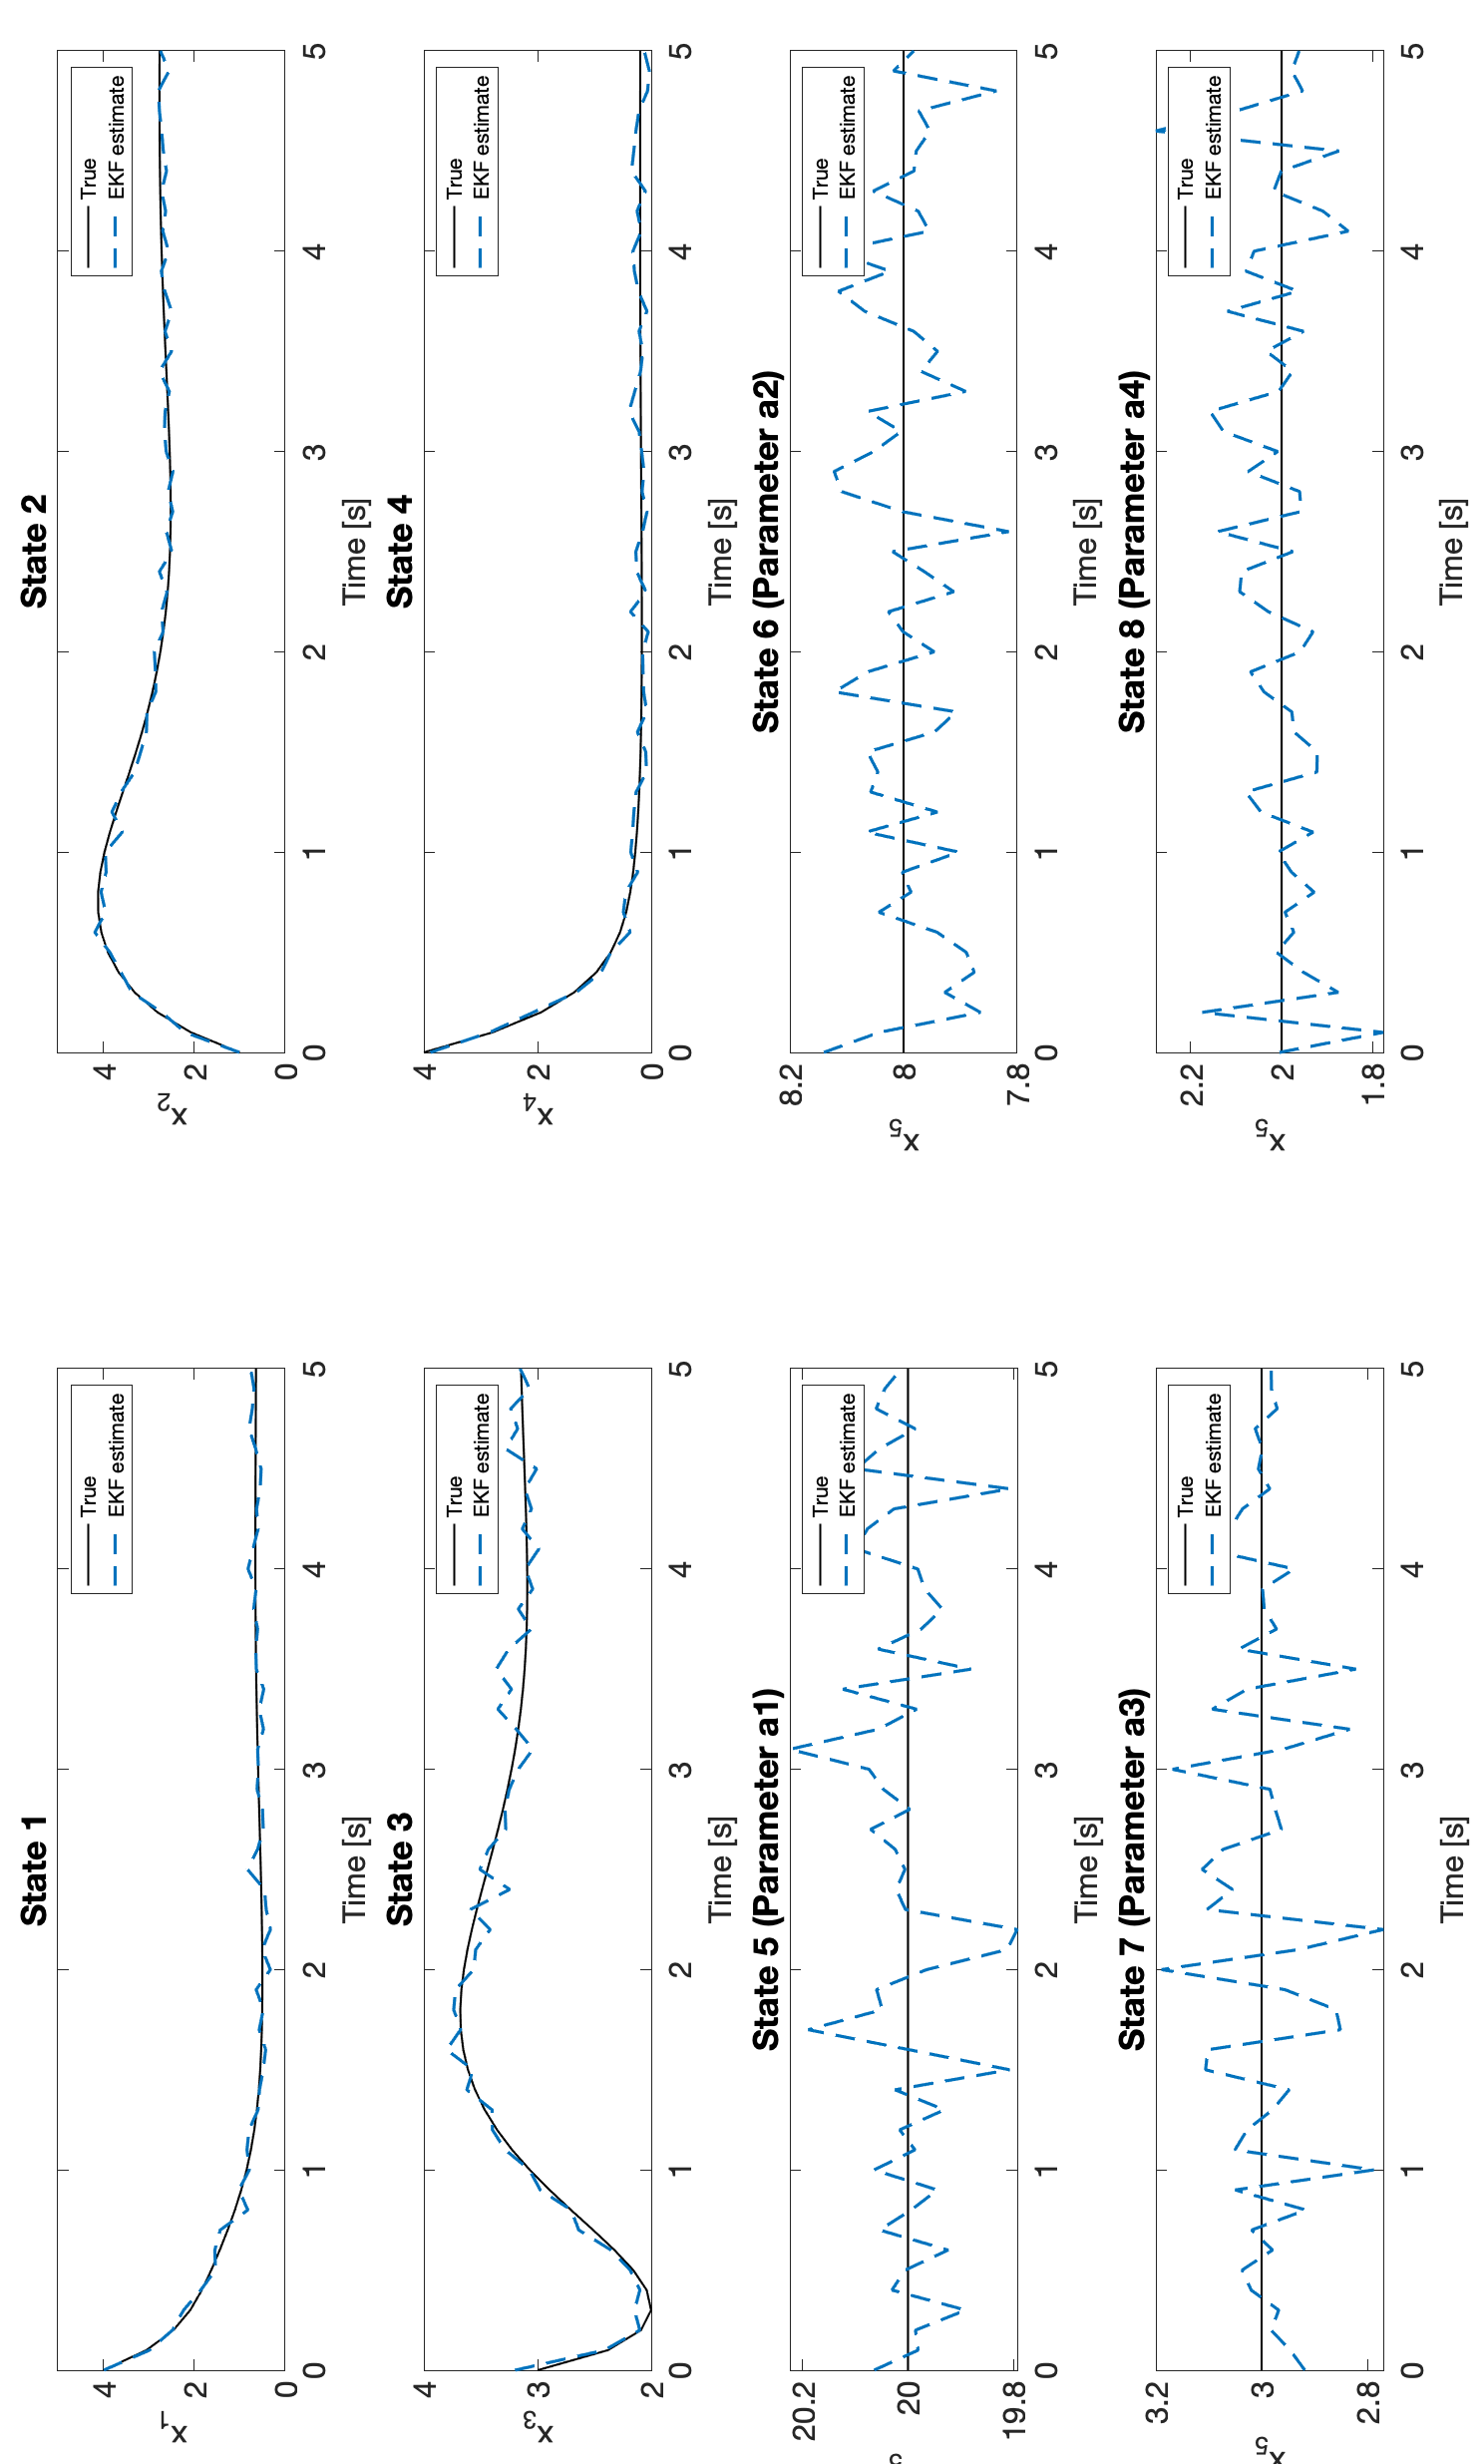
\includegraphics[scale = 0.5]{EKF_4param.png}
    \caption{EKF performance of an 8 state system with 4 parameters. This model was initialized with $[4;1;3;4;20;8;3;2]^T$, which is almost exactly the system's true values.}
    \label{fig:4param}
\end{figure}






\comment{
\noindent Residuals, also known as the innovation, are one way to access the model's performance. Recall that the residual is the difference between the actual measurement values and the predicted measurement values. Generally, a strong residual graph has

\begin{itemize}
\item a symmetrical distribution that is clustered toward the center,
\item values that are close to 0,
\item a random or unclear pattern.
\end{itemize}

\noindent Figure ~\ref{fig:4params} is the residual graph of the system where the EKF is applied to the four states and four parameters, $\alpha_1, \hdots, \alpha_4$. While this residual graph has values close to 0 and a symmetrical distribution, the pattern is similar to the behavior of the states. Therefore, though EKF can be applied to this nonlinear system, performance can be further optimized.

\begin{figure}[h]
    \centering
    \includegraphics[scale = 0.6]{EKF_4param_residual.png}
    \caption{Built in matlab, four state correction and 4 param}
    \label{fig:4params}
\end{figure}


\noindent There are many methods of parameter estimation, which include using dual techniques. In fact, there is a nonlinear version of the Kalman Filter, called the Dual Unscented Kalman Filter, that was designed in order to simultaneously monitor state and parameter values. Though this thesis does not explore these methods, more information can be found in \cite{inbook, article6}. 
}
















